\documentclass{article}
\usepackage{graphicx} % Required for inserting images
\usepackage{biblatex} %Imports biblatex package
\addbibresource{references.bib} %Import the bibliography file


\title{Preprint submission}
\author{Christian Magelssen}
\date{February 2024}

\begin{document}

\maketitle

\section{Introduction}

The hallmark of expertise lies in the flawless execution of actions and the selection of optimal choices to achieve goals  \cite{wolpert_principles_2011, krakauer_motor_2019, mangalam_investigating_2023, du_relationship_2022, gallivan_decision-making_2018}. These choices (or cognitive strategies) are typically trained with instruction-based approaches, where a coach tells learners what to do (e.g., take a shorter line around the gate) followed by corrective feedback (e.g., you can shorten the line even more) \cite{williams_practice_2005, williams_effective_2023, hodges_role_1999}. This teaching strategy can be likened to what motor learning refers to as supervised learning, where the teaching signal for skill improvement represents the disparity between the desired skill outcome and the learner outcome \cite{jordan_forward_1992, wolpert_motor_2010, doya_complementary_2000}. Through practice this teaching signal can bring the learner closer to execute what is assumed to be the correct choice, but does this teaching approach truly foster creativity and intelligent strategic choices, such as helping learners discover innovative and vastly more effective solutions that surpass our imagination?

One drawback of the supervised learning strategy for training these decisions is that learners are simply told what to do based on what coaches believe to be a good strategy from their knowledge or experience. However, what coaches judge as a good strategy does not always align with reality, even for the best-trained eye \cite{supej_impact_2019, cochrum_visual_2021}. Learners might, therefore, miss opportunities to discover the best strategy when coaches opt for suboptimal choices \cite{gray_plateaus_2017}. Supervised learning might also constrain learners to adopting a single ('universal') strategy for all situations rather than acquiring a repertoire of strategies and discerning the most effective strategies for each specific scenario. Finally, it remains uncertain whether the prescriptive approach is the most effective teaching strategy for achieving long-lasting learning effects \cite{wulf_instructions_1997} 

Learning to make good choices can also happen without the direct influence of a coach who gives advice. The cornerstone of reinforcement learning \cite{sutton_reinforcement_2018} is that learners can learn by exploring strategies and evaluating their outcomes, using the successes and failures of outcomes as teaching signals. That is, rather than being told the putatively correct solution to the problem, as in supervised learning, they learn about the value of different strategies, which allows them to pick the best solution. These values are learned by comparing a given choice's outcomes with the currently expected outcome of that choice. Outcomes that exceed or fall short of expectations result in errors in reward prediction, signaling that the learner must update their predictions to better anticipate future rewards following that action \cite{rescorla_theory_1972}. These reward prediction errors are then incorporated to form a new and better estimate of reward, by updating expectations through a weighted running average. Reinforcement learning has been tremendously powerful in explaining human and animal learning \cite{waelti_dopamine_2001, schultz_neural_1997, pessiglione_dopamine-dependent_2006}, as well as training AI to perform complex tasks such as computer games starting from pixel inputs, only\cite{mnih_human-level_2015}. Given this evidence, could reinforcement learning offer an alternative to standard coach-based supervised learning to improve strategy selection and performance for skilled performers?

Advancing strategy choices in elite performers, however, extends beyond merely selecting an effective strategy; it entails consistently seeking new and better methods, a defining characteristic of deliberate practice \cite{ericsson_development_2003, ericsson_expert_1994, ericsson_role_1993}. Sometimes, achieving substantial performance improvements requires making radical shifts in strategy choices \cite{taylor_role_2012, gray_plateaus_2017}. Such switches require learners to enter a deliberate mode of action selection where they reorganize their mental representation of the skill to come up with even better strategies and performance\cite{du_relationship_2022}. How learners decide on, learn, and develop strategies is not currently known\cite{taylor_role_2012}, especially not in expert performers. Our question was whether reinforcement learning could contribute to better strategy selection than traditional supervised learning by allowing learners to experiment with strategies and evaluate their effects. 

To address this question, we conducted a three-day learning experiment with ninety-eight skilled and elite alpine ski racers from Norway and Sweden. To facilitate skill development in this skilled group of athletes, we selected a section of a slalom course where there is great improvement potential, even among the best skiers. This skill was to improve times on flat sections in slalom, and we defined four strategies intentionally to enhance this skill (\ref{fig:courseandstrategies}b). Our hypothesis was that skiers in the reinforcement learning group would learn to choose better strategies and thus achieve better performance than skiers subject to traditional supervised learning with a coach. To test this, we assigned skiers to three different learning groups with different instructions and feedback (Fig. \ref{fig:experiment}b): In the reinforcement learning group, skiers chose a strategy on every run and saw their race times to inform these decisions. In the supervised (free choice) learning group, a ski coach made this choice for the skier, while in the supervised (target skill) learning group, we recruited current World-Cup ski coaches to instruct skiers to select the strategy that we defined as the theoretically best strategy based on computational modeling \cite{lind_physics_2013} and observations of elite skiers \cite{reid_alpine_2020}. Coaches in the two supervised learning groups saw the times but were instructed not to disclose them to the skiers. 

We found that the reinforcement learning group showed greater improvement during acquisition and performed better in retention compared to the supervised (free choice) learning group. We observed an improvement in strategy choices for both reinforcement learning and supervised (free choice) learning groups, but we did not observe any statistically significant differences in choices between groups, either for the theoretically best strategy or individual skiers' estimated best strategy. We also found that both groups were sensitive to performance feedback, exhibiting win-stay, lose-shift behavior in strategy choices, but the descriptively greater sensitivity to feedback in the reinforcement learning group was not statistically significant. Our results suggest that reinforcement learning yields comparable outcomes to supervised learning, and that any advantages of reinforcement learning over supervised learning are more likely rooted in effects on skill execution rather than action selection. 



\begin{figure}[h!]
\centering
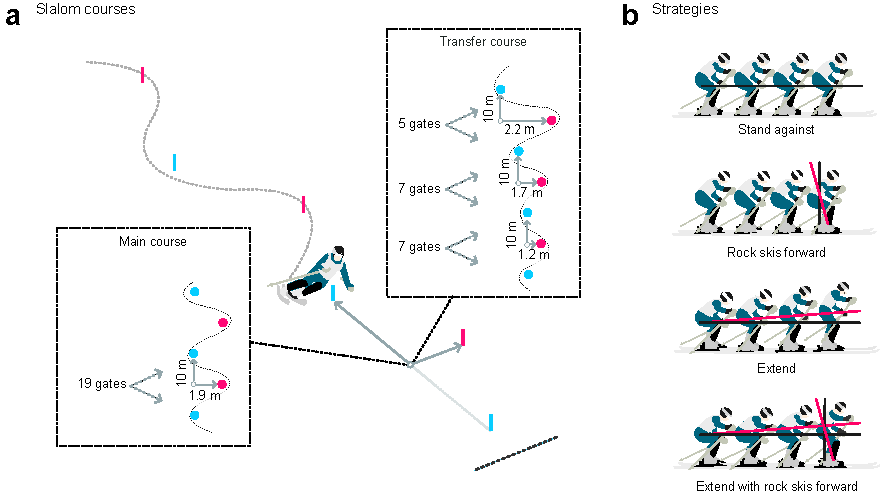
\includegraphics{figures/figure_method_courseandstrategy.pdf}
\caption{\textbf{a.} Illustrations of the two slalom courses used in the study. The main slalom course was a rhythmic course deployed in all sessions except for the transfer test. The course setting for the transfer test involved a progression in gate offset, starting with the largest offset and ending with the smallest offset. \textbf{b.} Illustration of the strategies defined to enhance racing performance on flat terrain in slalom: The "stand against" strategy emphasized maintaining a stable stance against external forces without body extension along the body's longitudinal axis or rocking skis forward; 'Rock skis forward' involved rocking skis forward from gate passage to completion of the turn; The "extend" strategy involves extending the body from a laterally tilted position during the turn, closer to the turn's center of rotation; The "extend with rocking skis forward" was expected to be the best strategy combining the two effects from extending and rocking skis forward, and we therefore defined this as the theoretical best strategy}
\label{fig:courseandstrategies}
\end{figure}

\begin{figure}[h!]
\centering
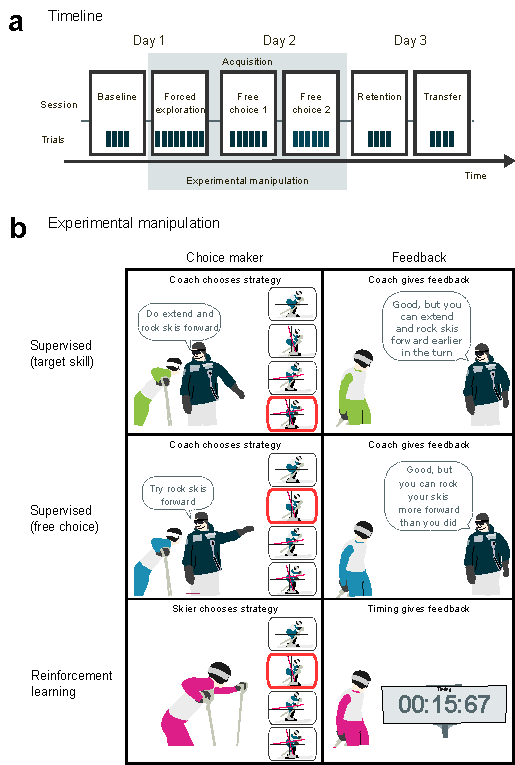
\includegraphics{figures/figure_method_experiment.pdf}
\caption{Illustration of the experimental design and procedure. \textbf{a.} Timeline of the three-day skill learning experiment. During the baseline, skiers skied a slalom course as fast as they could without receiving racing time feedback. The skiers' performances were ranked to form blocks. Within each block, skiers were randomly assigned to one of three treatment groups (see b).Skiers underwent an acquisition phase in their designated treatment group comprising one forced exploration and two free-choice sessions. On the last day, skiers completed a retention and transfer test, again without feedback from coaches nor timing. \textbf{b.} Illustration of treatment groups in the study. Supervised (target skill) involved coaches consistently choosing the theoretically best strategy, while supervised (free choice) allowed coaches to select strategies freely. Skiers in both these treatment groups received feedback on strategy execution from their respective coach, while skiers in the reinforcement learning group independently selected strategies and received feedback from the timing system to facilitate value learning of each strategy. }
\label{fig:experiment}
\end{figure}



\section{Discussion}

Expert performance relies on selecting and executing effective strategies with precision. The conventional method for training these decisions involves instructing learners on which strategy to choose. Our question was whether reinforcement learning could improve strategy selection and performance among adept alpine ski racers. Our findings indicate that reinforcement learning can complement traditional training methods and serve as a functional approach specifically tailored to train decision-making skills. We suggest that coaches can improve skill acquisition by crafting strategies and enabling learners to glean insights into their outcomes through evaluations rather than solely relying on direct instruction. 


\subsection{Race time}
Interestingly, the reinforcement learning group improved their race more during acquisition and had better retention than did the supervised (free-choice) learning group. This result accords first with prior studies on the 'discovery learning' approach, where practice without explicit instruction yields better learning effects \cite{wulf_instructions_1997, hodges_learning_2001}. More specifically, this finding aligns with earlier studies in reinforcement learning, which have demonstrated that learning through reinforcement feedback increases retention\cite{therrien_effective_2016, truong_error-based_2023, hasson_reinforcement_2015}. The presumed explanation behind these findings is that reinforcement enhances offline improvements in motor memories that are not observed with other learning paradigms. 

Although reinforcement learning also demonstrated descriptively better race times than supervised learning during the acquisition phase and retention, these differences were not significant. The strategy selected thus appeared to have been effective for this group. However, the advantage of using this strategy seemed to diminish over the course of the sessions, as this group experienced a descriptive decline from the first to the last free choice sessions in the acquisition phase. One possible explanation for this is that the strategy lost its effectiveness. We will discuss this more in..

Our hypothesis was also that reinforcement learning improves transfer to a new slalom course. The rationale for such expected behaviour was that reinforcement learning would achieve better insights into to the strategies' effect, thereby promoting better decision-making in new situations. However, we found no corroborating evidence for this hypothesis. This result aligns with studies that have observed enhanced retention but not transfer with reinforcement compared to supervised learning \cite{hasson_reinforcement_2015}. Furthermore, reinforcement learning has been found to yield a lower generalization signature in adaptive tasks \cite{lior_shmuelof_overcoming_2012}. One account for these findings is that reinforcement learning improves learning only for the specific situations in which one has been rewarded, as these are the instances in which learning has been reinforced. A potential mechanism for this is that training with rewards shortens the time window during which memory is unstable, affecting learners' capacity to extend learning to new situations \cite{robertson_memory_2018}. It is also conceivable that a more structured learning approach, where learners are exposed to frequent switches between strategies, is necessary to grasp the task's structure and promote transfer \cite{braun_structure_2010}. Future research should possibly investigate the effect of structural learning. 

\subsection{Choices and learning}
Our initial explanation for the improved acquisition and retention in the reinforcement learning group was that they learned to choose better strategies through evaluation via choice. During acquisition, we found that reinforcement learning enhanced its choices, while we did not observe the same evidence for supervised (free choice) learning. Both groups exhibited a 'win-stay, lose-switch' signature, indicating a tendency to stick to successful strategies. Despite reinforcement learning showing a descriptive tendency to select better strategies and having more pronounced "win-stay, lose-switch" tendencies during acquisition, these differences were not statistically significant, contrary to our initial hypothesis. 

Similar 'win-stay, lose-switch' tendencies have been found in other motor learning studies. The finding of 'win-stay, lose-switch' in our study suggests that elite sportspeople seek effective strategies. One plausible explanation for not finding corroborating evidence for group differences in choice or on 'win-stay, lose-switch' is that we were dealing with highly experienced coaches with solid sports knowledge. Therefore, we should be cautious in describing this as a null result. It is also important to note that coaches had access to skiers' race times and underwent significant learning too. In a typical training situation, coaches might not have tested strategies as extensively as in this study.  

A surprising finding was that supervised (free choice) learning had a descriptively higher predicted probability of choosing the skier's estimated best strategy on retention. Still, the reinforcement learning had the fastest race times during retention. One interpretation of this result is that skiers in the reinforcement learning group took into consideration the variability of performing a strategy and opted for those with lower incurred risk, despite another strategy being more effective. This understanding may have arisen because skiers in the reinforcement learning group discovered that multiple strategies led to similar outcomes and chose the slightly worse strategy due to lower variability. In that case, one might consider that "extend with rock skis forward" to be more risky since it could potentially make athletes lean too far backward to be able to engage the skis in the next turn. However, this does not seem to be a good account of our data as the choices of this strategy increased on retention. A more likely explanation is that that the skiers in reinforcement learning built a better mental representation of the strategies and learned that two or more produced the same outcomes, and just picked any of them.

This explanation, however, cannot fully account for the disparity in race time. Compared with supervised (free choice) learning, reinforcement learning achieved greater improvement in the 'extend' strategy, suggesting that reinforcement feedback might have increasing motor vigor \cite{pietro_mazzoni_why_2007, dudman_basal_2016}, such that their "energized" this action better. Indeed, previous studies have found that people make saccades \cite{takikawa_modulation_2002} and reach\cite{summerside_vigor_2018} faster towards targets paired with rewards than unpaired targets. Comments from a few coaches, who watched the retention and transfer, from the sideline, uttered that skiers in the reinforcement learning group used more forceful arm movements than skiers in the other groups, despite the instruction did not tell them to do that.

The vigor perspective may also help explaining why reinforcement learning did not learn better than the supervised (target skill) learning group, as previous studies also have found that training with explicit knowledge boosts motor vigor much like the effect of reward itself \cite{anderson_rewards_2020, wong_explicit_2015}. It may therefore be that the getting information from a current World Cup coach that one strategy was best boosted the implicit motivation to perform this strategy well. 


Our study suggests that reinforcement learning can be an essential training strategy to improve skill acquisition. However, before encouraging coaches and instructors to implement this strategy, we discuss the significance of the effect size and its amplifying and counteracting mechanisms for generalizability \cite{anvari_not_2023}. To start this discussion, we emphasize that the estimated effect size during retention was smaller than our predefined smallest effect size of interest. This benchmark, however, was set for a longer slalom course and more training sessions than we could execute due to space and time constraints in the ski hall. Consequently, we exercise caution in outright dismissing its practical significance. Instead, we aim to help the reader understand its potential importance for skill improvement in our sample of skiers. The first step towards this insight is to consider that the slalom course approximately equaled one-third of a full slalom race course, and a slalom race consists of two runs. Therefore, the 0.12 seconds effect size could be scaled up by a factor of 6, potentially proving significant for coaches in a more accurate course setup. However, racecourses consisting solely of flat sections are rare, and it is more realistic to assume that a flat section of a course constitutes only one-third of the entire course. If we base our understanding on this assumption, we can convert the 0.12-second difference into FIS world ranking positions. Considering that a race consists of two runs, this translates into an improved World Rank of 27 positions for females and 65 for males, based on a median ranking of 600 in our sample (see Supplement discussion). This could be of significant importance, but we have to remember that this effect cannot be directly transferred, as sports expertise also involves cognitive decisions \cite{mangalam_investigating_2023, krakauer_motor_2019}, such as switching from one strategy to another during a race. Our study did not capture such decisions as we focused on flat sections. In conclusion, the estimated effect could be larger if not because reinforcement learning and supervised learning conducted the retention and transfer tests simultaneously. This design choice allowed the skiers to observe each other, possibly diluting some of the effect. However, this decision was made to mirror the conditions of alpine competitions and gave us confidence that athletes experienced similar conditions during testing. 

\section{Methods}

\subsection{Participants}
We recruited ten alpine ski teams from Norway and Sweden, comprising
98alpine ski racers (age \textit{M} = 18.1, \textit{SD }= 2;  40 female,  58 male). Two skiers were excluded from the analysis due to an injury prior to the study (\textit{n}=1) and sickness during the study (\textit{n}=1), leaving us with a total of 96 skiers completed the entire åstudy and were included for the analysis. We deliberately opted to recruit skiers with diverse skill levels for the study to augment the generalizability of our findings. However, to ensure a sufficient skill level to handle the specific icy snow conditions prepared in the skiing hall, we only recruited skiers aged 15 and older. Among the ski groups that were tested were five ski academies, three senior development teams, and two national ski teams. These skiers were generally highly skilled, with a median world rank of 605, but there was also considerable variability, as indicated by a substantial interquartile range (Q1 = 248, Q3 = 1390.5). A smaller subset of the participants (n = 13) was not world-ranked, as they had yet to record FIS points. Table 1 provides demographic information for each treatment group.






\end{document}
